% Options for packages loaded elsewhere
\PassOptionsToPackage{unicode}{hyperref}
\PassOptionsToPackage{hyphens}{url}
%
\documentclass[
]{book}
\usepackage{amsmath,amssymb}
\usepackage{iftex}
\ifPDFTeX
  \usepackage[T1]{fontenc}
  \usepackage[utf8]{inputenc}
  \usepackage{textcomp} % provide euro and other symbols
\else % if luatex or xetex
  \usepackage{unicode-math} % this also loads fontspec
  \defaultfontfeatures{Scale=MatchLowercase}
  \defaultfontfeatures[\rmfamily]{Ligatures=TeX,Scale=1}
\fi
\usepackage{lmodern}
\ifPDFTeX\else
  % xetex/luatex font selection
\fi
% Use upquote if available, for straight quotes in verbatim environments
\IfFileExists{upquote.sty}{\usepackage{upquote}}{}
\IfFileExists{microtype.sty}{% use microtype if available
  \usepackage[]{microtype}
  \UseMicrotypeSet[protrusion]{basicmath} % disable protrusion for tt fonts
}{}
\makeatletter
\@ifundefined{KOMAClassName}{% if non-KOMA class
  \IfFileExists{parskip.sty}{%
    \usepackage{parskip}
  }{% else
    \setlength{\parindent}{0pt}
    \setlength{\parskip}{6pt plus 2pt minus 1pt}}
}{% if KOMA class
  \KOMAoptions{parskip=half}}
\makeatother
\usepackage{xcolor}
\usepackage{color}
\usepackage{fancyvrb}
\newcommand{\VerbBar}{|}
\newcommand{\VERB}{\Verb[commandchars=\\\{\}]}
\DefineVerbatimEnvironment{Highlighting}{Verbatim}{commandchars=\\\{\}}
% Add ',fontsize=\small' for more characters per line
\usepackage{framed}
\definecolor{shadecolor}{RGB}{248,248,248}
\newenvironment{Shaded}{\begin{snugshade}}{\end{snugshade}}
\newcommand{\AlertTok}[1]{\textcolor[rgb]{0.94,0.16,0.16}{#1}}
\newcommand{\AnnotationTok}[1]{\textcolor[rgb]{0.56,0.35,0.01}{\textbf{\textit{#1}}}}
\newcommand{\AttributeTok}[1]{\textcolor[rgb]{0.13,0.29,0.53}{#1}}
\newcommand{\BaseNTok}[1]{\textcolor[rgb]{0.00,0.00,0.81}{#1}}
\newcommand{\BuiltInTok}[1]{#1}
\newcommand{\CharTok}[1]{\textcolor[rgb]{0.31,0.60,0.02}{#1}}
\newcommand{\CommentTok}[1]{\textcolor[rgb]{0.56,0.35,0.01}{\textit{#1}}}
\newcommand{\CommentVarTok}[1]{\textcolor[rgb]{0.56,0.35,0.01}{\textbf{\textit{#1}}}}
\newcommand{\ConstantTok}[1]{\textcolor[rgb]{0.56,0.35,0.01}{#1}}
\newcommand{\ControlFlowTok}[1]{\textcolor[rgb]{0.13,0.29,0.53}{\textbf{#1}}}
\newcommand{\DataTypeTok}[1]{\textcolor[rgb]{0.13,0.29,0.53}{#1}}
\newcommand{\DecValTok}[1]{\textcolor[rgb]{0.00,0.00,0.81}{#1}}
\newcommand{\DocumentationTok}[1]{\textcolor[rgb]{0.56,0.35,0.01}{\textbf{\textit{#1}}}}
\newcommand{\ErrorTok}[1]{\textcolor[rgb]{0.64,0.00,0.00}{\textbf{#1}}}
\newcommand{\ExtensionTok}[1]{#1}
\newcommand{\FloatTok}[1]{\textcolor[rgb]{0.00,0.00,0.81}{#1}}
\newcommand{\FunctionTok}[1]{\textcolor[rgb]{0.13,0.29,0.53}{\textbf{#1}}}
\newcommand{\ImportTok}[1]{#1}
\newcommand{\InformationTok}[1]{\textcolor[rgb]{0.56,0.35,0.01}{\textbf{\textit{#1}}}}
\newcommand{\KeywordTok}[1]{\textcolor[rgb]{0.13,0.29,0.53}{\textbf{#1}}}
\newcommand{\NormalTok}[1]{#1}
\newcommand{\OperatorTok}[1]{\textcolor[rgb]{0.81,0.36,0.00}{\textbf{#1}}}
\newcommand{\OtherTok}[1]{\textcolor[rgb]{0.56,0.35,0.01}{#1}}
\newcommand{\PreprocessorTok}[1]{\textcolor[rgb]{0.56,0.35,0.01}{\textit{#1}}}
\newcommand{\RegionMarkerTok}[1]{#1}
\newcommand{\SpecialCharTok}[1]{\textcolor[rgb]{0.81,0.36,0.00}{\textbf{#1}}}
\newcommand{\SpecialStringTok}[1]{\textcolor[rgb]{0.31,0.60,0.02}{#1}}
\newcommand{\StringTok}[1]{\textcolor[rgb]{0.31,0.60,0.02}{#1}}
\newcommand{\VariableTok}[1]{\textcolor[rgb]{0.00,0.00,0.00}{#1}}
\newcommand{\VerbatimStringTok}[1]{\textcolor[rgb]{0.31,0.60,0.02}{#1}}
\newcommand{\WarningTok}[1]{\textcolor[rgb]{0.56,0.35,0.01}{\textbf{\textit{#1}}}}
\usepackage{longtable,booktabs,array}
\usepackage{calc} % for calculating minipage widths
% Correct order of tables after \paragraph or \subparagraph
\usepackage{etoolbox}
\makeatletter
\patchcmd\longtable{\par}{\if@noskipsec\mbox{}\fi\par}{}{}
\makeatother
% Allow footnotes in longtable head/foot
\IfFileExists{footnotehyper.sty}{\usepackage{footnotehyper}}{\usepackage{footnote}}
\makesavenoteenv{longtable}
\usepackage{graphicx}
\makeatletter
\def\maxwidth{\ifdim\Gin@nat@width>\linewidth\linewidth\else\Gin@nat@width\fi}
\def\maxheight{\ifdim\Gin@nat@height>\textheight\textheight\else\Gin@nat@height\fi}
\makeatother
% Scale images if necessary, so that they will not overflow the page
% margins by default, and it is still possible to overwrite the defaults
% using explicit options in \includegraphics[width, height, ...]{}
\setkeys{Gin}{width=\maxwidth,height=\maxheight,keepaspectratio}
% Set default figure placement to htbp
\makeatletter
\def\fps@figure{htbp}
\makeatother
\setlength{\emergencystretch}{3em} % prevent overfull lines
\providecommand{\tightlist}{%
  \setlength{\itemsep}{0pt}\setlength{\parskip}{0pt}}
\setcounter{secnumdepth}{5}
\usepackage{booktabs}
\usepackage[numbers]{natbib}
\setcitestyle{numbers,square}
\ifLuaTeX
  \usepackage{selnolig}  % disable illegal ligatures
\fi
\usepackage[]{natbib}
\bibliographystyle{plainnat}
\IfFileExists{bookmark.sty}{\usepackage{bookmark}}{\usepackage{hyperref}}
\IfFileExists{xurl.sty}{\usepackage{xurl}}{} % add URL line breaks if available
\urlstyle{same}
\hypersetup{
  pdftitle={Code for Quantitative Bias Analysis},
  pdfauthor={Jeremy Brown},
  hidelinks,
  pdfcreator={LaTeX via pandoc}}

\title{Code for Quantitative Bias Analysis}
\author{Jeremy Brown}
\date{}

\begin{document}
\maketitle

{
\setcounter{tocdepth}{1}
\tableofcontents
}
\hypertarget{about}{%
\chapter{About}\label{about}}

This site contains code for the \protect\hyperlink{applied-examples}{applied examples} in the article ``\emph{Quantifying possible bias in clinical and epidemiological studies using quantitative bias analysis}'' in addition to illustrative code to conduct alternative quantitative bias analyses.

\hypertarget{applied-examples}{%
\chapter{Applied examples}\label{applied-examples}}

In ``\emph{Applying quantitative bias analysis in clinical and epidemiological studies using quantitative bias analysis}'' we present three applied examples of bias formulas, bounding methods, and probabilistic bias analysis. Code to generate results for these applied examples is presented below.

\hypertarget{bias-formulas-for-selection-bias}{%
\section{Bias formulas for selection bias}\label{bias-formulas-for-selection-bias}}

In a cohort study of pregnant women investigating the association between maternal lithium use, relative to non-use, and cardiac malformations in live-born infants, a covariate-adjusted risk ratio was estimated of 1.65 (95\% CI, 1.02-2.68).\citep{patorno2017lithium} Live-born infants only were included in the study and as such there was potential for selection bias if there were differences in termination probabilities of foetuses with cardiac malformations by exposure group.

Given that the outcome was rare, and therefore odds ratios and risk ratios are approximately equivalent, bias formulas using odds ratios were applied.\citep{greenland1996basic}

\[
OR_{BiasAdjusted} = OR_{Observed}\frac{S_{01}S_{10}}{S_{00}S_{11}}
\]
Values for the bias parameters, selection probabilities by exposure and outcome status, were specified based on the literature. The selection probability of unexposed without cardiac malformations was assumed to be 0.8 (i.e.~20\% probability of termination). The selection probability of unexposed with cardiac malformation was varied from 0.5 to 0.7. (30-50\% probability of termination). Selection probabilities of exposed were defined by outcome status relative to unexposed (0\% to -10\%).

\begin{Shaded}
\begin{Highlighting}[]
\FunctionTok{library}\NormalTok{(tidyverse)}
\FunctionTok{library}\NormalTok{(ggplot2)}

\CommentTok{\# Define observed odds ratio}
\NormalTok{observed\_rr }\OtherTok{\textless{}{-}} \FloatTok{1.65}

\CommentTok{\# Define bias parameters}
\NormalTok{S00 }\OtherTok{\textless{}{-}} \FloatTok{0.8}
\NormalTok{S01 }\OtherTok{\textless{}{-}} \FunctionTok{c}\NormalTok{(}\FloatTok{0.5}\NormalTok{, }\FloatTok{0.525}\NormalTok{, }\FloatTok{0.55}\NormalTok{, }\FloatTok{0.575}\NormalTok{, }\FloatTok{0.6}\NormalTok{, }\FloatTok{0.625}\NormalTok{, }\FloatTok{0.65}\NormalTok{, }\FloatTok{0.675}\NormalTok{, }\FloatTok{0.7}\NormalTok{)}
\NormalTok{differences }\OtherTok{\textless{}{-}} \FunctionTok{c}\NormalTok{(}\DecValTok{0}\NormalTok{, }\SpecialCharTok{{-}}\FloatTok{0.05}\NormalTok{, }\SpecialCharTok{{-}}\FloatTok{0.1}\NormalTok{) }

\CommentTok{\# Define function to calculate bias{-}adjusted risk ratio}
\NormalTok{calc\_bias\_adj\_or }\OtherTok{\textless{}{-}} \ControlFlowTok{function}\NormalTok{(or, s01, s10, s00, s11) \{}
\NormalTok{  bias\_adj\_or }\OtherTok{\textless{}{-}}\NormalTok{ or }\SpecialCharTok{*}\NormalTok{ (s01}\SpecialCharTok{*}\NormalTok{s10)}\SpecialCharTok{/}\NormalTok{(s00}\SpecialCharTok{*}\NormalTok{s11)}
  \FunctionTok{return}\NormalTok{(bias\_adj\_or)}
\NormalTok{\}}

\CommentTok{\# Calculate bias{-}adjusted estimate for different values of bias parameters}
\NormalTok{results }\OtherTok{\textless{}{-}} \ConstantTok{NULL}
\ControlFlowTok{for}\NormalTok{ (s01 }\ControlFlowTok{in}\NormalTok{ S01) \{}
  \ControlFlowTok{for}\NormalTok{ (diff }\ControlFlowTok{in}\NormalTok{ differences) \{}
\NormalTok{    bias\_adj\_rr }\OtherTok{\textless{}{-}} \FunctionTok{calc\_bias\_adj\_or}\NormalTok{(observed\_rr, s01, S00 }\SpecialCharTok{+}\NormalTok{ diff, S00, s01 }\SpecialCharTok{+}\NormalTok{ diff)}
\NormalTok{    results\_row }\OtherTok{\textless{}{-}} \FunctionTok{tibble\_row}\NormalTok{(}\AttributeTok{bias\_adj\_rr=}\NormalTok{bias\_adj\_rr, }\AttributeTok{s01=}\NormalTok{s01, }\AttributeTok{diff=}\FunctionTok{as.character}\NormalTok{(diff))}
\NormalTok{    results }\OtherTok{\textless{}{-}} \FunctionTok{bind\_rows}\NormalTok{(results, results\_row)}
\NormalTok{  \}}
\NormalTok{\}}

\CommentTok{\# Tidy label for difference in selection probabilities}
\NormalTok{results }\OtherTok{\textless{}{-}}\NormalTok{ results }\SpecialCharTok{\%\textgreater{}\%} 
  \FunctionTok{mutate}\NormalTok{(}\AttributeTok{diff=}\FunctionTok{factor}\NormalTok{(diff, }\AttributeTok{levels=}\FunctionTok{c}\NormalTok{(}\StringTok{"0"}\NormalTok{, }\StringTok{"{-}0.05"}\NormalTok{, }\StringTok{"{-}0.1"}\NormalTok{), }\AttributeTok{labels=}\FunctionTok{c}\NormalTok{(}\StringTok{"0"}\NormalTok{, }\StringTok{"{-}5\%"}\NormalTok{, }\StringTok{"{-}10\%"}\NormalTok{)))}

\CommentTok{\# Plot figure of bias{-}adjusted estimates}
\FunctionTok{ggplot}\NormalTok{(}\AttributeTok{data =}\NormalTok{ results, }\FunctionTok{aes}\NormalTok{(}\AttributeTok{x=}\NormalTok{s01, }\AttributeTok{y=}\NormalTok{bias\_adj\_rr, }\AttributeTok{colour=}\NormalTok{diff)) }\SpecialCharTok{+} 
  \FunctionTok{geom\_line}\NormalTok{() }\SpecialCharTok{+} 
  \FunctionTok{theme\_minimal}\NormalTok{() }\SpecialCharTok{+}
  \FunctionTok{ylim}\NormalTok{(}\FloatTok{1.4}\NormalTok{, }\DecValTok{2}\NormalTok{) }\SpecialCharTok{+} 
  \FunctionTok{scale\_x\_reverse}\NormalTok{() }\SpecialCharTok{+}
  \FunctionTok{xlab}\NormalTok{(}\StringTok{"Selection probability of unexposed with cardiac malformations"}\NormalTok{) }\SpecialCharTok{+} 
  \FunctionTok{ylab}\NormalTok{(}\StringTok{"Bias{-}adjusted risk ratio"}\NormalTok{) }\SpecialCharTok{+}
  \FunctionTok{guides}\NormalTok{(}\AttributeTok{colour=}\FunctionTok{guide\_legend}\NormalTok{(}\AttributeTok{title=}\StringTok{"Difference in selection}\SpecialCharTok{\textbackslash{}n}\StringTok{probability of exposed"}\NormalTok{)) }\SpecialCharTok{+}
  \FunctionTok{theme}\NormalTok{(}\AttributeTok{legend.title=}\FunctionTok{element\_text}\NormalTok{(}\AttributeTok{size=}\DecValTok{10}\NormalTok{))}
\end{Highlighting}
\end{Shaded}

\begin{figure}

{\centering 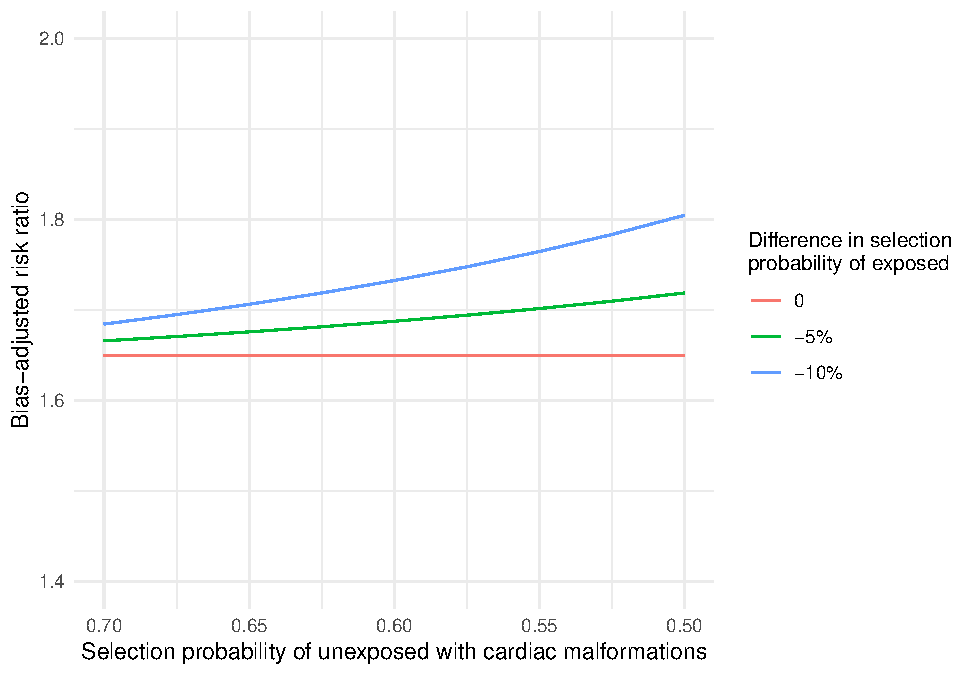
\includegraphics{_main_files/figure-latex/bias-adj-1} 

}

\caption{Bias-adjusted risk ratio for different assumed selection probabilities}\label{fig:bias-adj}
\end{figure}

The bias-adjusted risk ratios ranged from 1.65 to 1.80 (Figure \ref{fig:bias-adj}), indicating robustness of the point estimate to selection bias under the given assumptions. We can likewise calculate bias-adjusted estimates for the lower bound of the confidence interval.

\textbackslash begin\{figure\}

\{\centering 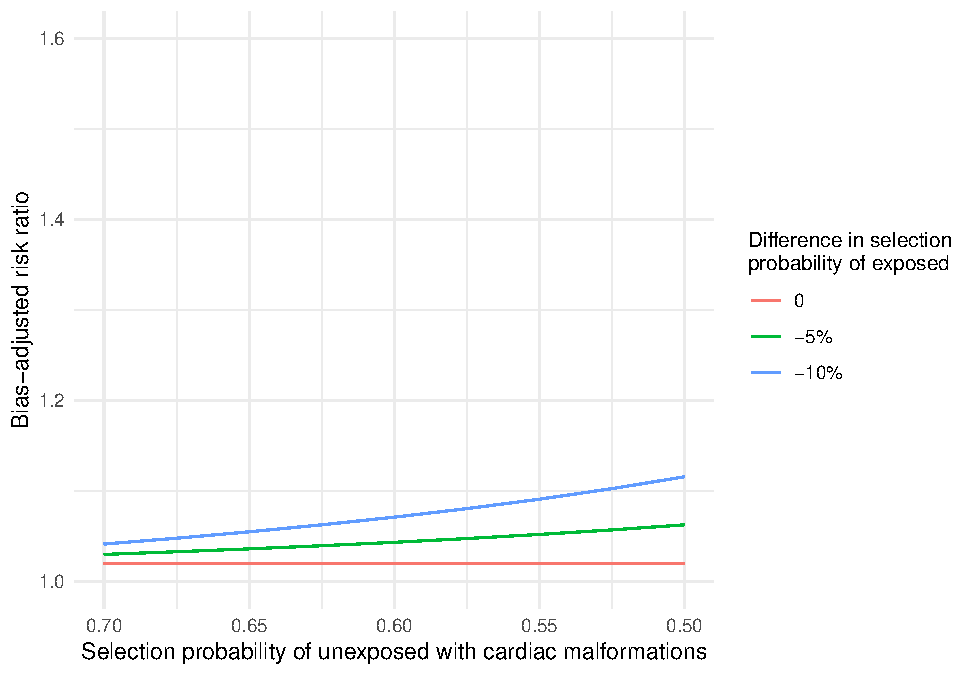
\includegraphics{_main_files/figure-latex/bias-adj-lb-1}

\}

\textbackslash caption\{Bias-adjusted risk ratio for lower bound of 95\% confidence interval for different assumed selection probabilities\}\label{fig:bias-adj-lb}
\textbackslash end\{figure\}

\hypertarget{e-values-for-unmeasured-confounding}{%
\section{E-values for unmeasured confounding}\label{e-values-for-unmeasured-confounding}}

In a cohort study conducted in electronic health records investigating the association between proton pump inhibitors, relative to H2 receptor antagonists, and all-cause mortality, investigators found that individuals were at higher risk of death (covariate-adjusted hazard ratio {[}HR{]} 1.38, 95\% CI 1.33-1.44).\citep{brown2021proton} However, it was considered that there may be unmeasured confounding due to differences in frailty between individuals prescribed proton pump inhibitors. The prevalence of the unmeasured confounder was not known in either exposure group, and therefore rather than use bias formulas, an E-value was calculated.\citep{ding2016sensitivity}

Given the outcome was rare, the E-value method can be applied to the hazard ratio.

\[
\text{E-value} = RR_{Obs} + \sqrt{RR_{Obs}(RR_{Obs} -1)}
\]

We can use the \href{https://cran.r-project.org/web/packages/EValue/index.html}{EValue} package to calculate E-Values.

\begin{Shaded}
\begin{Highlighting}[]
\CommentTok{\# load EValue package and ggplotify }
\FunctionTok{library}\NormalTok{(EValue)}

\CommentTok{\#Calculate E{-}values}
\FunctionTok{evalues.HR}\NormalTok{(}\AttributeTok{est=}\FloatTok{1.38}\NormalTok{, }\AttributeTok{lo=}\FloatTok{1.33}\NormalTok{, }\AttributeTok{hi=}\FloatTok{1.44}\NormalTok{, }\AttributeTok{rare=}\ConstantTok{TRUE}\NormalTok{) }\SpecialCharTok{\%\textgreater{}\%}\NormalTok{  knitr}\SpecialCharTok{::}\FunctionTok{kable}\NormalTok{()}
\end{Highlighting}
\end{Shaded}

\begin{tabular}{l|r|r|r}
\hline
  & point & lower & upper\\
\hline
RR & 1.380000 & 1.330000 & 1.44\\
\hline
E-values & 2.104155 & 1.992495 & NA\\
\hline
\end{tabular}

And we can use \emph{bias\_plot} from the \emph{EValue} package to display an E-value plot.

\begin{Shaded}
\begin{Highlighting}[]
\CommentTok{\# Generate E{-}value plot for point estimate}
\FunctionTok{bias\_plot}\NormalTok{(}\FloatTok{1.38}\NormalTok{, }\AttributeTok{xmax=}\DecValTok{9}\NormalTok{) }
\end{Highlighting}
\end{Shaded}

\begin{figure}

{\centering 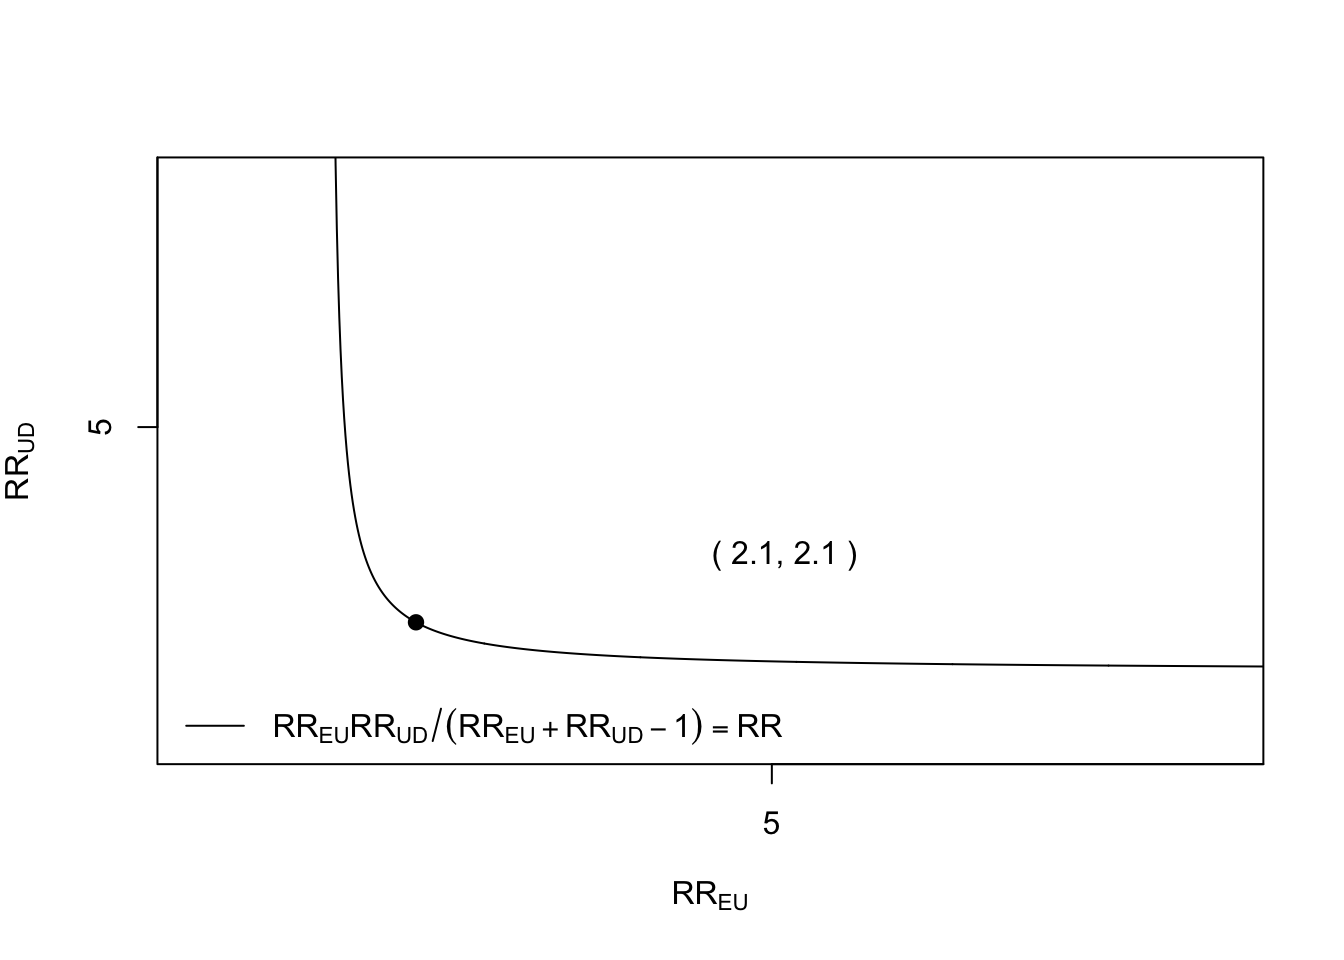
\includegraphics{_main_files/figure-latex/unnamed-chunk-3-1} 

}

\caption{E-value plot for point estimate}\label{fig:unnamed-chunk-3}
\end{figure}

The E-value for the point estimate was 2.10 and for the lower bound of the point estimate was 1.99. This represents the minimum strength of association that an unmeasured confounder would need to have with either exposure or outcome to reduce the hazard ratio to the null (i.e.~1). An unmeasured confounder with strength of association with exposure and outcome below the line in the plot could not possibly explain, on its own, the observed association.

Risk ratios between frailty and mortality \textgreater2 have been observed in the literature, and as such we could not rule out unmeasured confounding as a possible explanation for findings based on the E-value. However, as we did not specify prevalence of an unmeasured confounder, we cannot say whether such confounding was likely to account for the observed association. There may also have been additional unmeasured or partially measured confounders contributing to the observed association.

\hypertarget{probabilistic-bias-analysis-for-misclassification}{%
\section{Probabilistic bias analysis for misclassification}\label{probabilistic-bias-analysis-for-misclassification}}

In a cohort study of pregnant women conducted using insurance claims data, the observed covariate-adjusted risk ratio for the association between antidepressant use and congenital cardiac defects, was 1.02 (95\% CI, 0.90-1.15).\citep{huybrechts2014antidepressant} Some misclassification of the outcome, congenital cardiac malformation was anticipated. Therefore, probabilistic bias analysis was carried out.\citep{fox2005method} Code is not provided for this analysis, which was carrier out using SAS and participant record-level data (see \href{https://sites.google.com/site/biasanalysis/sensmac}{sensmac} macro for a SAS program to conduct this analysis).

\begin{figure}

{\centering 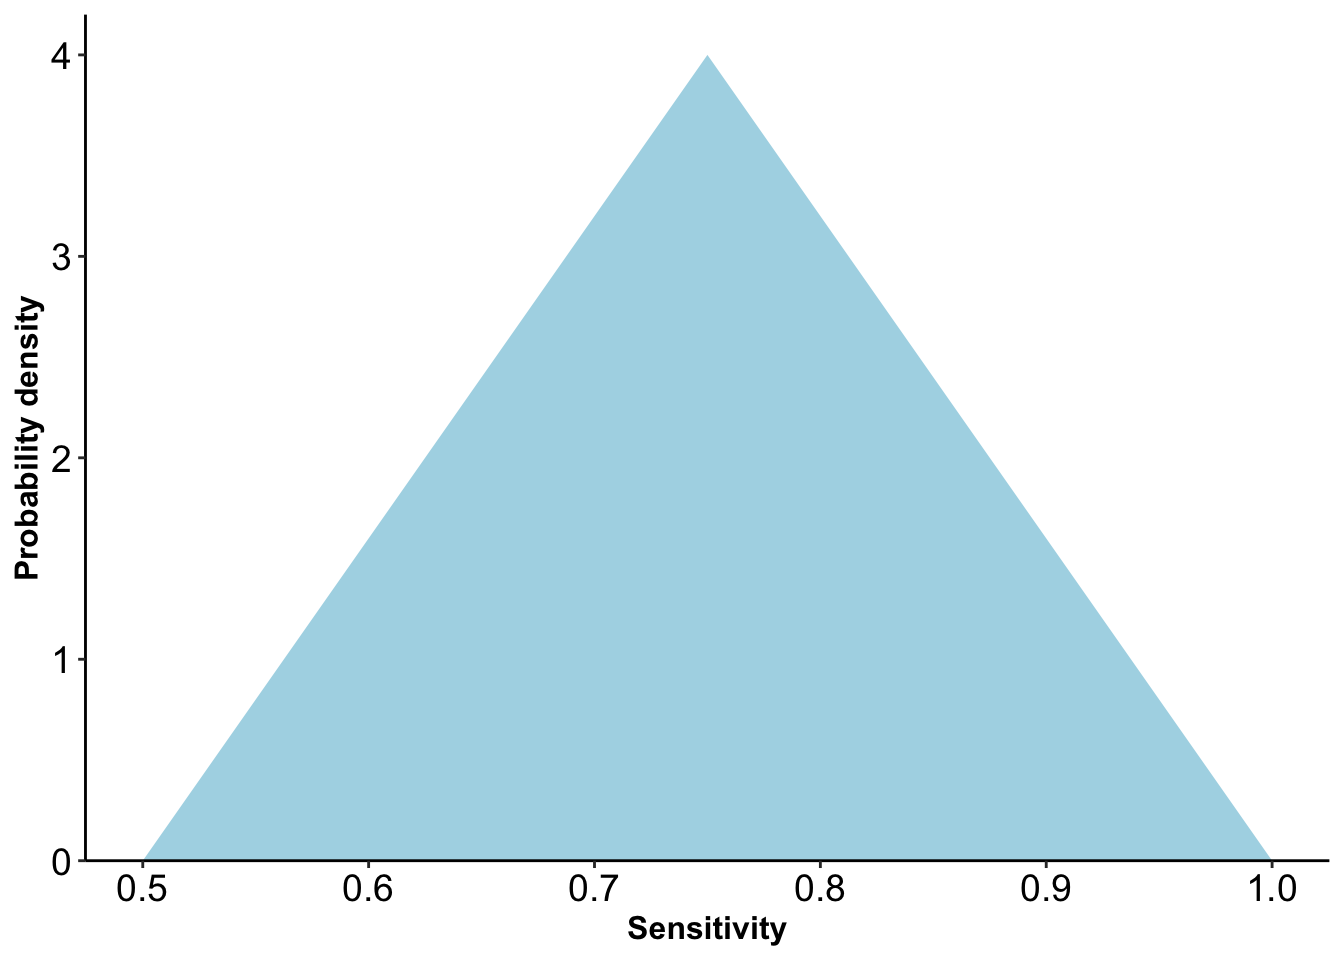
\includegraphics[width=0.6\linewidth]{_main_files/figure-latex/triangular-1} 

}

\caption{Triangular distribution for sensitivity}\label{fig:triangular}
\end{figure}

Positive predictive values estimated in a validation study were used to specify distributions of values for the bias parameters of sensitivity and specificity. Investigators chose triangular distributions for the positive and negative predictive value (Figure \ref{fig:triangular}).

Values were repeatedly sampled at random 1,000 times from these distributions and these sampled values were used to calculate a distribution of bias-adjusted estimates. The median bias-adjusted estimate was 1.06 with 95\% simulation interval 0.92-1.22.

\hypertarget{additional-examples}{%
\chapter{Additional example applications}\label{additional-examples}}

We will present here examples of quantitative bias analysis using simulated participant-level data for a cohort study with a binary treatment, binary outcome, and binary confounder.

\begin{Shaded}
\begin{Highlighting}[]
\CommentTok{\# load packages}
\FunctionTok{require}\NormalTok{(tidyverse)}
\FunctionTok{require}\NormalTok{(ggplot2)}
\FunctionTok{library}\NormalTok{(broom) }
\FunctionTok{library}\NormalTok{(janitor)}
\end{Highlighting}
\end{Shaded}

\hypertarget{selection-bias}{%
\section{Selection bias}\label{selection-bias}}

In the simulated data we have a binary treatment \(a\), binary confounder \(x\), outcome \(y\), and a binary indicator for selection into the study \(s\).

\begin{Shaded}
\begin{Highlighting}[]
\NormalTok{sim\_data }\OtherTok{\textless{}{-}} \FunctionTok{read\_csv}\NormalTok{(}\StringTok{"data/simulated\_data.csv"}\NormalTok{) }\SpecialCharTok{\%\textgreater{}\%} \FunctionTok{select}\NormalTok{(x,a,y,s)}
\NormalTok{sim\_data  }\SpecialCharTok{\%\textgreater{}\%} \FunctionTok{head}\NormalTok{(}\DecValTok{5}\NormalTok{)}
\end{Highlighting}
\end{Shaded}

\begin{verbatim}
## # A tibble: 5 x 4
##       x     a     y     s
##   <dbl> <dbl> <dbl> <dbl>
## 1     0     0     0     1
## 2     0     0     0     1
## 3     0     0     0     1
## 4     0     0     0     1
## 5     0     0     0     1
\end{verbatim}

The data was generated such that the causal odds ratio between treatment and outcome was 2. However, in a given sample the estimate may differ due to random error. If we observed a random sample from the target population we could unbiasedly estimate the odds ratio using logistic regression.

\begin{Shaded}
\begin{Highlighting}[]
\CommentTok{\# fit logistic regression model}
\NormalTok{lgr\_model }\OtherTok{\textless{}{-}} \FunctionTok{glm}\NormalTok{(y }\SpecialCharTok{\textasciitilde{}}\NormalTok{ x }\SpecialCharTok{+}\NormalTok{ a, }\AttributeTok{data=}\NormalTok{sim\_data, }\AttributeTok{family=}\StringTok{"binomial"}\NormalTok{) }

\CommentTok{\# tidy model outputs}
\NormalTok{or }\OtherTok{\textless{}{-}}\NormalTok{ lgr\_model }\SpecialCharTok{\%\textgreater{}\%} 
  \FunctionTok{tidy}\NormalTok{(}\AttributeTok{exponentiate=}\ConstantTok{TRUE}\NormalTok{, }\AttributeTok{conf.int=}\ConstantTok{TRUE}\NormalTok{) }\SpecialCharTok{\%\textgreater{}\%} 
  \FunctionTok{filter}\NormalTok{(term }\SpecialCharTok{==} \StringTok{"a"}\NormalTok{) }\SpecialCharTok{\%\textgreater{}\%} 
  \FunctionTok{select}\NormalTok{(estimate, conf.low, conf.high)}

\CommentTok{\# output as table}
\NormalTok{or }\SpecialCharTok{\%\textgreater{}\%} 
\NormalTok{  knitr}\SpecialCharTok{::}\FunctionTok{kable}\NormalTok{(}\AttributeTok{caption =} \StringTok{"Estimated odds ratio"}\NormalTok{)}
\end{Highlighting}
\end{Shaded}

\begin{table}

\caption{\label{tab:unnamed-chunk-7}Estimated odds ratio}
\centering
\begin{tabular}[t]{r|r|r}
\hline
estimate & conf.low & conf.high\\
\hline
2.040021 & 1.942229 & 2.142647\\
\hline
\end{tabular}
\end{table}

However, if we consider that selection into the study was dependent on exposure and outcome and that we only observed a selected subsample of the target population, then the estimated odds ratio is biased.

\begin{Shaded}
\begin{Highlighting}[]
\CommentTok{\# restrict data to selected subsample}
\NormalTok{selected\_data }\OtherTok{\textless{}{-}}\NormalTok{ sim\_data }\SpecialCharTok{\%\textgreater{}\%} \FunctionTok{filter}\NormalTok{(s }\SpecialCharTok{==} \DecValTok{1}\NormalTok{)}

\CommentTok{\# fit logistic regression model}
\NormalTok{lgr\_model\_selected }\OtherTok{\textless{}{-}} \FunctionTok{glm}\NormalTok{(y }\SpecialCharTok{\textasciitilde{}}\NormalTok{ x }\SpecialCharTok{+}\NormalTok{ a, }\AttributeTok{data=}\NormalTok{selected\_data, }\AttributeTok{family=}\StringTok{"binomial"}\NormalTok{) }

\CommentTok{\# tidy model outputs}
\NormalTok{or\_selected }\OtherTok{\textless{}{-}}\NormalTok{ lgr\_model\_selected }\SpecialCharTok{\%\textgreater{}\%} 
  \FunctionTok{tidy}\NormalTok{(}\AttributeTok{exponentiate=}\ConstantTok{TRUE}\NormalTok{, }\AttributeTok{conf.int=}\ConstantTok{TRUE}\NormalTok{) }\SpecialCharTok{\%\textgreater{}\%} 
  \FunctionTok{filter}\NormalTok{(term }\SpecialCharTok{==} \StringTok{"a"}\NormalTok{) }\SpecialCharTok{\%\textgreater{}\%} 
  \FunctionTok{select}\NormalTok{(estimate, conf.low, conf.high) }

\CommentTok{\# output as table}
\NormalTok{or\_selected }\SpecialCharTok{\%\textgreater{}\%}
\NormalTok{  knitr}\SpecialCharTok{::}\FunctionTok{kable}\NormalTok{(}\AttributeTok{caption =} \StringTok{"Estimated odds ratio in selected sample"}\NormalTok{)}
\end{Highlighting}
\end{Shaded}

\begin{table}

\caption{\label{tab:unnamed-chunk-8}Estimated odds ratio in selected sample}
\centering
\begin{tabular}[t]{r|r|r}
\hline
estimate & conf.low & conf.high\\
\hline
1.577843 & 1.494616 & 1.665406\\
\hline
\end{tabular}
\end{table}

\hypertarget{bias-formulas}{%
\subsection{Bias formulas}\label{bias-formulas}}

One option is to apply bias formulas for the odds ratio.

\[
OR_{BiasAdjusted} = OR_{Observed}\frac{S_{01}S_{10}}{S_{00}S_{11}}
\]
Given that the data was simulated we know the selection probabilities (\(S11=0.7\), \(S01=1\), \(S10=0.9\), \(S00=1\)) and can directly plug them in to estimate a bias-adjusted odds ratio. However, in practice we will not know these probabilities and will typically specify a range of values, or for probabilistic bias analysis a distribution of values.

\begin{Shaded}
\begin{Highlighting}[]
\CommentTok{\# define bias parameters}
\NormalTok{S11 }\OtherTok{\textless{}{-}} \FloatTok{0.7}
\NormalTok{S01 }\OtherTok{\textless{}{-}} \DecValTok{1}
\NormalTok{S10 }\OtherTok{\textless{}{-}} \FloatTok{0.9}
\NormalTok{S00 }\OtherTok{\textless{}{-}} \DecValTok{1}

\CommentTok{\# apply bias formula}
\NormalTok{bias\_adjusted\_or }\OtherTok{\textless{}{-}}\NormalTok{ or\_selected }\SpecialCharTok{\%\textgreater{}\%} 
  \FunctionTok{mutate}\NormalTok{(}\FunctionTok{across}\NormalTok{(}\FunctionTok{c}\NormalTok{(estimate, conf.low, conf.high), }\SpecialCharTok{\textasciitilde{}}\NormalTok{ .x }\SpecialCharTok{*}\NormalTok{ (S01}\SpecialCharTok{*}\NormalTok{S10)}\SpecialCharTok{/}\NormalTok{(S11}\SpecialCharTok{*}\NormalTok{S00)))}

\CommentTok{\# output as table}
\NormalTok{bias\_adjusted\_or }\SpecialCharTok{\%\textgreater{}\%} 
\NormalTok{  knitr}\SpecialCharTok{::}\FunctionTok{kable}\NormalTok{(}\AttributeTok{caption =} \StringTok{"Bias{-}adjusted odds ratio"}\NormalTok{)}
\end{Highlighting}
\end{Shaded}

\begin{table}

\caption{\label{tab:unnamed-chunk-9}Bias-adjusted odds ratio}
\centering
\begin{tabular}[t]{r|r|r}
\hline
estimate & conf.low & conf.high\\
\hline
2.028656 & 1.92165 & 2.141236\\
\hline
\end{tabular}
\end{table}

\hypertarget{weighting}{%
\subsection{Weighting}\label{weighting}}

Alternatively, we can weight the individual records by the inverse probability of selection and use bootstapping to calculate a confidence interval

\begin{Shaded}
\begin{Highlighting}[]
\FunctionTok{library}\NormalTok{(boot)}

\CommentTok{\# Add weights}
\NormalTok{selected\_data\_with\_weights }\OtherTok{\textless{}{-}}\NormalTok{ selected\_data }\SpecialCharTok{\%\textgreater{}\%} 
  \FunctionTok{mutate}\NormalTok{(}\AttributeTok{prob\_select =}\NormalTok{ a}\SpecialCharTok{*}\NormalTok{y}\SpecialCharTok{*}\NormalTok{S11 }\SpecialCharTok{+}\NormalTok{ (}\DecValTok{1}\SpecialCharTok{{-}}\NormalTok{a)}\SpecialCharTok{*}\NormalTok{y}\SpecialCharTok{*}\NormalTok{S01 }\SpecialCharTok{+}\NormalTok{ a}\SpecialCharTok{*}\NormalTok{(}\DecValTok{1}\SpecialCharTok{{-}}\NormalTok{y)}\SpecialCharTok{*}\NormalTok{S10 }\SpecialCharTok{+}\NormalTok{ (}\DecValTok{1}\SpecialCharTok{{-}}\NormalTok{a)}\SpecialCharTok{*}\NormalTok{(}\DecValTok{1}\SpecialCharTok{{-}}\NormalTok{y)}\SpecialCharTok{*}\NormalTok{S00) }\SpecialCharTok{\%\textgreater{}\%}
  \FunctionTok{mutate}\NormalTok{(}\AttributeTok{inverse\_prob =} \DecValTok{1}\SpecialCharTok{/}\NormalTok{prob\_select) }

\CommentTok{\# define function to estimate weighted odds ratio (needed for bootstrap function)}
\NormalTok{calculate\_weighted\_or }\OtherTok{\textless{}{-}} \ControlFlowTok{function}\NormalTok{(weighted\_data, i) \{}
\NormalTok{  weighted\_lgr }\OtherTok{\textless{}{-}} \FunctionTok{glm}\NormalTok{(y }\SpecialCharTok{\textasciitilde{}}\NormalTok{ x }\SpecialCharTok{+}\NormalTok{ a, }\AttributeTok{family=}\StringTok{"binomial"}\NormalTok{, }\AttributeTok{data=}\NormalTok{weighted\_data[i,], }\AttributeTok{weights=}\NormalTok{inverse\_prob) }
\NormalTok{  weighted\_or }\OtherTok{\textless{}{-}} \FunctionTok{coef}\NormalTok{(weighted\_lgr)[[}\StringTok{"a"}\NormalTok{]] }\SpecialCharTok{\%\textgreater{}\%} \FunctionTok{exp}\NormalTok{()}
  \FunctionTok{return}\NormalTok{(weighted\_or)}
\NormalTok{\}}

\CommentTok{\# set seed of random number generator to ensure reproducibility}
\FunctionTok{set.seed}\NormalTok{(}\DecValTok{747}\NormalTok{)}

\CommentTok{\# bootstrap calculation of confidence intervals}
\NormalTok{bootstrap\_estimates }\OtherTok{\textless{}{-}} \FunctionTok{boot}\NormalTok{(selected\_data\_with\_weights, calculate\_weighted\_or, }\AttributeTok{R=}\DecValTok{1000}\NormalTok{)}

\CommentTok{\# calculate bias{-}adjusted point estimate using entire selected subsample}
\NormalTok{point\_estimate }\OtherTok{\textless{}{-}} \FunctionTok{calculate\_weighted\_or}\NormalTok{(selected\_data\_with\_weights, }\DecValTok{1}\SpecialCharTok{:}\FunctionTok{nrow}\NormalTok{(selected\_data\_with\_weights))}

\CommentTok{\# calculate percentile bootstrap confidence interval}
\NormalTok{conf\_int }\OtherTok{\textless{}{-}} \FunctionTok{quantile}\NormalTok{(bootstrap\_estimates}\SpecialCharTok{$}\NormalTok{t, }\FunctionTok{c}\NormalTok{(}\FloatTok{0.025}\NormalTok{, }\FloatTok{0.975}\NormalTok{))}

\CommentTok{\# output bias{-}adjusted estimate}
\FunctionTok{tibble}\NormalTok{(}\AttributeTok{estimate=}\NormalTok{point\_estimate, }\AttributeTok{conf.low=}\NormalTok{conf\_int[[}\DecValTok{1}\NormalTok{]], }\AttributeTok{conf.high=}\NormalTok{conf\_int[[}\DecValTok{2}\NormalTok{]]) }\SpecialCharTok{\%\textgreater{}\%}
\NormalTok{  knitr}\SpecialCharTok{::}\FunctionTok{kable}\NormalTok{()}
\end{Highlighting}
\end{Shaded}

If we expect selection probabilities to differ within levels of covariates then we can specify different selection probabilities for different strata of covariates.

\hypertarget{misclassification}{%
\section{Misclassification}\label{misclassification}}

We will now consider some quantitative bias analysis methods for misclassification of a binary outcome. Similar approaches can be applied for misclassification of a binary exposure.

With differential misclassification of the outcome, \(m_y\), the odds ratio is biased.

\begin{Shaded}
\begin{Highlighting}[]
\CommentTok{\# load data}
\NormalTok{misclassified\_data }\OtherTok{\textless{}{-}} \FunctionTok{read\_csv}\NormalTok{(}\StringTok{"data/simulated\_data.csv"}\NormalTok{) }\SpecialCharTok{\%\textgreater{}\%} \FunctionTok{select}\NormalTok{(x,a,m\_y,s)}

\CommentTok{\# fit logistic regression model with misclassified outcome}
\NormalTok{lgr\_model\_misclassified }\OtherTok{\textless{}{-}} \FunctionTok{glm}\NormalTok{(m\_y }\SpecialCharTok{\textasciitilde{}}\NormalTok{ x }\SpecialCharTok{+}\NormalTok{ a, }\AttributeTok{data=}\NormalTok{misclassified\_data, }\AttributeTok{family=}\StringTok{"binomial"}\NormalTok{) }

\CommentTok{\# tidy model outputs}
\NormalTok{or\_misclassified }\OtherTok{\textless{}{-}}\NormalTok{ lgr\_model\_misclassified }\SpecialCharTok{\%\textgreater{}\%} 
  \FunctionTok{tidy}\NormalTok{(}\AttributeTok{exponentiate=}\ConstantTok{TRUE}\NormalTok{, }\AttributeTok{conf.int=}\ConstantTok{TRUE}\NormalTok{) }\SpecialCharTok{\%\textgreater{}\%} 
  \FunctionTok{filter}\NormalTok{(term }\SpecialCharTok{==} \StringTok{"a"}\NormalTok{) }\SpecialCharTok{\%\textgreater{}\%} 
  \FunctionTok{select}\NormalTok{(estimate, conf.low, conf.high) }

\CommentTok{\# output as table}
\NormalTok{or\_misclassified }\SpecialCharTok{\%\textgreater{}\%}
\NormalTok{  knitr}\SpecialCharTok{::}\FunctionTok{kable}\NormalTok{(}\AttributeTok{caption =} \StringTok{"Estimated odds ratio with misclassified outcome"}\NormalTok{)}
\end{Highlighting}
\end{Shaded}

\begin{table}

\caption{\label{tab:unnamed-chunk-11}Estimated odds ratio with misclassified outcome}
\centering
\begin{tabular}[t]{r|r|r}
\hline
estimate & conf.low & conf.high\\
\hline
1.737071 & 1.650733 & 1.827756\\
\hline
\end{tabular}
\end{table}

\hypertarget{bias-formulas-1}{%
\subsection{Bias formulas}\label{bias-formulas-1}}

Bias formulas for misclassification typically apply to 2x2 tables or 2x2 tables stratified by covariates and require us to specify the bias parameters of sensitivity and specificity. Given that the data was simulated, we know that sensitivity and specificity among the treated were 80\% and 99\%, and that sensitivity and specificity among the unexposed were 100\%. In practice, we do not know these values, but can estimate them using validation studies and specify a range or, for probabilistic bias analysis, distribution of plausible values.

\begin{tabular}{l|l|l}
\hline
  & A.1 & A.0\\
\hline
Y*=1 & a & b\\
\hline
Y*=0 & c & d\\
\hline
\end{tabular}

\begin{Shaded}
\begin{Highlighting}[]
\CommentTok{\# create 2x2 table stratified by confounder}
\NormalTok{two\_by\_two }\OtherTok{\textless{}{-}}\NormalTok{ misclassified\_data }\SpecialCharTok{\%\textgreater{}\%} \FunctionTok{tabyl}\NormalTok{(m\_y,a, x) }\SpecialCharTok{\%\textgreater{}\%} \FunctionTok{adorn\_title}\NormalTok{()}

\CommentTok{\# 2x2 among those without the confounder}
\FunctionTok{print}\NormalTok{(}\StringTok{"Without confounder"}\NormalTok{)}
\end{Highlighting}
\end{Shaded}

\begin{verbatim}
## [1] "Without confounder"
\end{verbatim}

\begin{Shaded}
\begin{Highlighting}[]
\NormalTok{two\_by\_two[[}\DecValTok{1}\NormalTok{]] }
\end{Highlighting}
\end{Shaded}

\begin{verbatim}
##          a      
##  m_y     0     1
##    0 57291 18078
##    1  2982  1720
\end{verbatim}

\begin{Shaded}
\begin{Highlighting}[]
\CommentTok{\# 2x2 among those with the confounder}
\FunctionTok{print}\NormalTok{(}\StringTok{"With confounder"}\NormalTok{)}
\end{Highlighting}
\end{Shaded}

\begin{verbatim}
## [1] "With confounder"
\end{verbatim}

\begin{Shaded}
\begin{Highlighting}[]
\NormalTok{two\_by\_two[[}\DecValTok{2}\NormalTok{]] }
\end{Highlighting}
\end{Shaded}

\begin{verbatim}
##         a     
##  m_y    0    1
##    0 9138 8503
##    1  932 1356
\end{verbatim}

\begin{Shaded}
\begin{Highlighting}[]
\CommentTok{\# specify bias parameters}
\NormalTok{sensitivity\_a0 }\OtherTok{\textless{}{-}}  \DecValTok{1}
\NormalTok{sensitivity\_a1 }\OtherTok{\textless{}{-}} \FloatTok{0.8}
\NormalTok{specificity\_a0 }\OtherTok{\textless{}{-}} \DecValTok{1}
\NormalTok{specificity\_a1 }\OtherTok{\textless{}{-}} \FloatTok{0.99}

\CommentTok{\# define function to correct 2x2 table}
\NormalTok{correct\_two\_by\_two }\OtherTok{\textless{}{-}} \ControlFlowTok{function}\NormalTok{(a, b, c, d, sensitivity\_a0, sensitivity\_a1, specificity\_a0, specificity\_a1) \{}
  
\NormalTok{\}}

\CommentTok{\# extract values from 2x2 tables}
\NormalTok{a\_x0 }\OtherTok{\textless{}{-}}\NormalTok{ two\_by\_two[[}\DecValTok{1}\NormalTok{]][}\DecValTok{3}\NormalTok{,}\DecValTok{3}\NormalTok{] }\SpecialCharTok{\%\textgreater{}\%} \FunctionTok{as.integer}\NormalTok{()}
\NormalTok{b\_x0 }\OtherTok{\textless{}{-}}\NormalTok{ two\_by\_two[[}\DecValTok{1}\NormalTok{]][}\DecValTok{2}\NormalTok{,}\DecValTok{3}\NormalTok{] }\SpecialCharTok{\%\textgreater{}\%} \FunctionTok{as.integer}\NormalTok{()}
\NormalTok{c\_x0 }\OtherTok{\textless{}{-}}\NormalTok{ two\_by\_two[[}\DecValTok{1}\NormalTok{]][}\DecValTok{3}\NormalTok{,}\DecValTok{2}\NormalTok{] }\SpecialCharTok{\%\textgreater{}\%} \FunctionTok{as.integer}\NormalTok{()}
\NormalTok{d\_x0 }\OtherTok{\textless{}{-}}\NormalTok{ two\_by\_two[[}\DecValTok{1}\NormalTok{]][}\DecValTok{3}\NormalTok{,}\DecValTok{3}\NormalTok{] }\SpecialCharTok{\%\textgreater{}\%} \FunctionTok{as.integer}\NormalTok{()}
\NormalTok{a\_x1 }\OtherTok{\textless{}{-}}\NormalTok{ two\_by\_two[[}\DecValTok{2}\NormalTok{]][}\DecValTok{2}\NormalTok{,}\DecValTok{2}\NormalTok{] }\SpecialCharTok{\%\textgreater{}\%} \FunctionTok{as.integer}\NormalTok{()}
\NormalTok{b\_x1 }\OtherTok{\textless{}{-}}\NormalTok{ two\_by\_two[[}\DecValTok{2}\NormalTok{]][}\DecValTok{2}\NormalTok{,}\DecValTok{3}\NormalTok{] }\SpecialCharTok{\%\textgreater{}\%} \FunctionTok{as.integer}\NormalTok{()}
\NormalTok{c\_x1 }\OtherTok{\textless{}{-}}\NormalTok{ two\_by\_two[[}\DecValTok{2}\NormalTok{]][}\DecValTok{3}\NormalTok{,}\DecValTok{2}\NormalTok{] }\SpecialCharTok{\%\textgreater{}\%} \FunctionTok{as.integer}\NormalTok{()}
\NormalTok{d\_x1 }\OtherTok{\textless{}{-}}\NormalTok{ two\_by\_two[[}\DecValTok{2}\NormalTok{]][}\DecValTok{3}\NormalTok{,}\DecValTok{3}\NormalTok{] }\SpecialCharTok{\%\textgreater{}\%} \FunctionTok{as.integer}\NormalTok{()}

\CommentTok{\# correct 2x2 table }
\FunctionTok{correct\_two\_by\_two}\NormalTok{(a\_x0, b\_x0, c\_x0, d\_x0, sensitivity\_a0, sensitivity\_a1, specificity\_a0, specificity\_a1)}
\end{Highlighting}
\end{Shaded}

\begin{verbatim}
## NULL
\end{verbatim}

\begin{Shaded}
\begin{Highlighting}[]
\CommentTok{\# calculate }
\end{Highlighting}
\end{Shaded}

\hypertarget{record-level-correction}{%
\subsection{Record-level correction}\label{record-level-correction}}

\hypertarget{probabalistic-bias-analysis}{%
\subsection{Probabalistic bias analysis}\label{probabalistic-bias-analysis}}

\hypertarget{unmeasured-confounding}{%
\section{Unmeasured confounding}\label{unmeasured-confounding}}

  \bibliography{book.bib}

\end{document}
